\section{Результаты и обсуждение}

\subsection{Наработка ДНК-библиотек для последующих транформаций}

Для проведения трансформаций нужно было амплифицировать нужные плазмиды и геномные библиотеки дрожжей. Причем, при размножении библиотек важно было не потерять разнообразие фрагментов.


%Поэтому, в качестве метода трансформации бактерий была выбрана электропорация, так как этот способ является самым эффективным по количеству клонов с одной аликвоты клеток \cite{hanahan_plasmid_1991}.
%Для наработки плазмид и плазмидных библиотек использовались культуры E.coli штамм XL1 Blue (см. \ref{subsec:strains}).

Нужно было подготовить компетентные клетки для электропорации, которые бы эффективно трансформировались плазмидами (см. \ref{subsec:bac_comp}). 
%Были подготовлены электро-компетентные клетки. 
Полученные клетки были проверены контрольной транформацией плазмидой pYES2 с известной концентрацией. 
%С одной аликвоты компетентных клеток и 10 пикограмм ДНК было получено порядка нескольких сотен клонов. 
Эффективность полученных клеток составляла $10^7-10^8$клонов/мкг~ДНК, что  достаточно для размножения геномных библиотек дрожжей.

%Основная плазмида p426GALaSynGFP была наработана в E.coli и выделена с помощью лизиса щелочью и спиртового переосаждения (раздел\ref{subsec:bac_plasm_pur}). Чистота и концентрация плазмиды были проверены с помощью рестрикции (HindIII, SpeI, HindIII и SpeI, PvuII) и анализа на геле. 

%Плазмидные библиотеки, оверэкспрессионная и делеционная, были наработаны в E.coli. Геномные библиотеки представлены огромным набором фрагментов ДНК, гораздо б\'{о}льшим, чем число клонов дрожжей, которые необходимо получить, чтобы покрыть все участки генома с вероятностью 99.99\%. Это демонстрирует таблица~\ref{table:libs} (строка число независимых рекомбинантов) (раздел \ref{subsec:libs}). 

Во избежание обеднения библиотеки при амплификации мы выращивали трансформированных бактерий на твердой среде, что позволяло подсчитать число колоний. Выборку более 100\,000 клонов считали достаточной, так как число различных фрагментов ДНК, представленных в библиотеках составляет порядка $10^4-10^5$ (таблица~\ref{table:libs}).


%Выделенные библиотеки проверялись рестрикцией (оверэкспрессионная Eco32, делеционная NotI) и гель-электрофорезом. 

Дальнейшие опыты показали, что выделенной ДНК достаточно, чтобы покрыть геномы штаммов в скринингах --  описание в таблице~\ref{table:libs2}. 
В результате, было было наработано необходимое количество ДНК-библиотек без потери разнообразия фрагментов для проведения скринингов.


\begin{table}[h] \small
	\caption{Характеристика полученных растворов плазмидных библиотек}
	\label{table:libs2}
	\begin{tabular}{
			p{0.25\width- \tabcolsep} 
			p{0.1\width- 2\tabcolsep}
			p{0.15\width - 2\tabcolsep}
			p{0.3\width - 2\tabcolsep}
			p{0.2\width - \tabcolsep}}
	\graytable
	\toprule
	Библиотека & Объем, мкл & Концен-трация, мкг/мл & Эффективность трансформаций, клонов/мкл & Необходимо трансформантов для покрытия генома\\
	\midrule
	Оверэкспрессионная &
		300&0.2& 
		\pbox[t]{0.3\width}{300\gray{(W303/\textalpha Syn)} \\ 
		200 \gray{(cdc53-1/\textalpha Syn)}} & 
		\pbox[t]{20cm}{$1.0\times10^4$ \\ $1.0\times10^4$}
		\\
	Делеционная &
		300&
		0.1-0.2&
		200 \gray{(W303/\textalpha Syn)} & $3.0\times10^4$
		\\
	\bottomrule
	\end{tabular}
\end{table}


\subsection{Подготовка штаммов дрожжей дикого типа и температурно-чувствительных, индуцибельно экспрессирующих α-синуклеин}

Моделирование действия α-синуклеина мы планировали проводить на двух моделях -- дрожжах дикого типа и температурно-чувствительном мутанте cdc53-1, который можно аррестовать в фазе G\textsubscript{0} клеточного цикла. Было необходимо подготовить штаммы, содержащие плазмиду p426GALaSynGFP, (1) в которых экспрессия α-синуклеина бы эффективно индуцировалась на галактозной среде, (2) α-синуклеин бы образовывал типичные включения, (3) α-синуклеин был бы токсичен и заметно замедлял рост колоний, так как это бы позволило обозначить критерий отбора для дальнейшего скрининга, (4) которые бы эффективно трансформировались выбранными геномными библиотеками.

%Дрожжи дикого типа W303 и температурно-чувствительный штамм cdc53-1 были трансформированы плазмидой p426GALaSynGFP по литий-ацетатному протоколу (см. \ref{subsec:yeast_trans}).

Эффективность индукции экспресии α-синуклеина, характеристика включений оценивалась по распределению GFP в клетках под флюоресцентным микроскопом. Клоны с селективной чашки подращивались на глюкозе, а затем на галактозе индуцировался синтез α-синуклеина в течении 24 часов. Отбирался клон с наибольшей долей экспрессирующих GFP клеток и для которого экспрессия синуклеина токсична.

%Отдельно, на галактозе оценивалась скорость роста клонов. Клоны отличались, так как процедура трансформации подразумевает клеточный стресс и перестройку, что может привести к каким-либо мутациям, изменениям эпигеномного контекста в клоне, что влияет на выживаемость при экспрессии белка. Выбирался клон, для которого экспрессия синуклеина токсична.

%Были получены штаммы W303/αSyn и cdc53-1/αSyn.

Отобранные штаммы W303/αSyn и cdc53-1/αSyn, действительно, при культивировании в одинаковых условиях, давали меньшее число видимых колоний при росте на галактозе по сравнению с глюкозой, колонии были мельче. % что демострирует рисунок~\ref{fig:compare}. 
Микроскопия показала, что на галактозе многие клетки начинают делиться, но рост останавливается после 5-10 делений, что демострирует рисунок~\ref{fig:division}.

%Мы наблюдали заметную разницу в скорости и качестве роста штамма W303/αSyn на индуцирующей среде (с галактозой), по сравнению с тем же штаммом  W303/αSyn на обычной среде (с глюкозой) либо штаммом W303:URA3, который содержит функционирующий ген URA3 в геноме, на селективной среде без урацила, но с галактозой. 

%Таким образом, в качестве критерия первичного отбора при скрининге, мы могли использовать качественную оценку роста колоний в сравнении в приведенными вариантами контроля. Нашим критерием отбора было образование больших колоний после введения библиотеки.

\begin{figure*}[h]
	\centering
	\begin{subfigure}[t]{0.49\textwidth}
		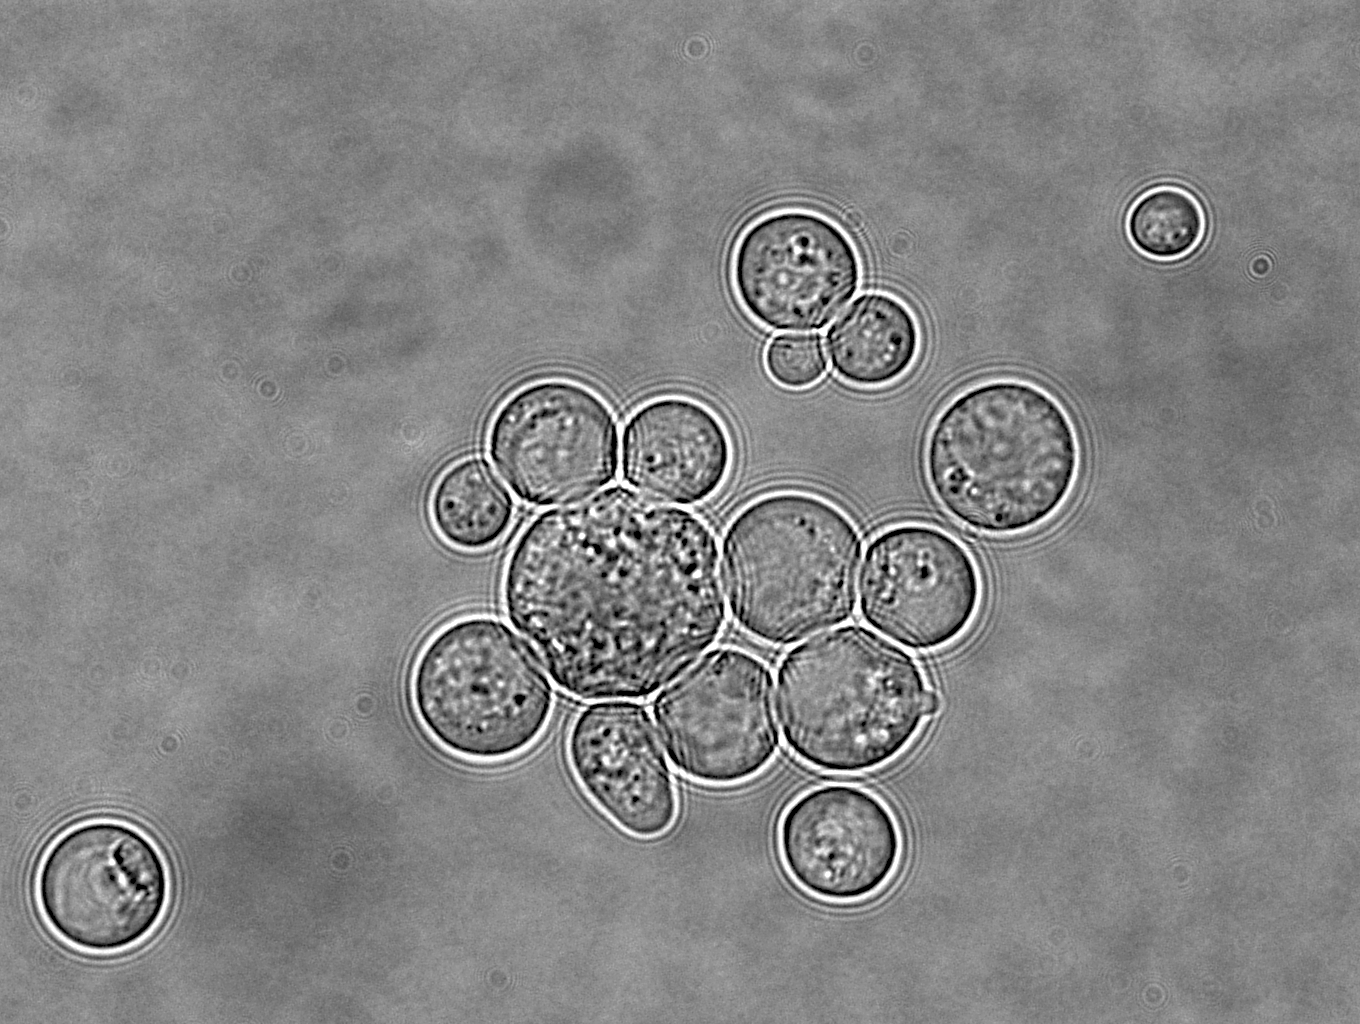
\includegraphics[width = \textwidth]{pics/1246_5hrs_GAL-4-0.png}
		\caption{DIC}\label{fig:}

	\end{subfigure}
	\begin{subfigure}[t]{0.49\linewidth}
		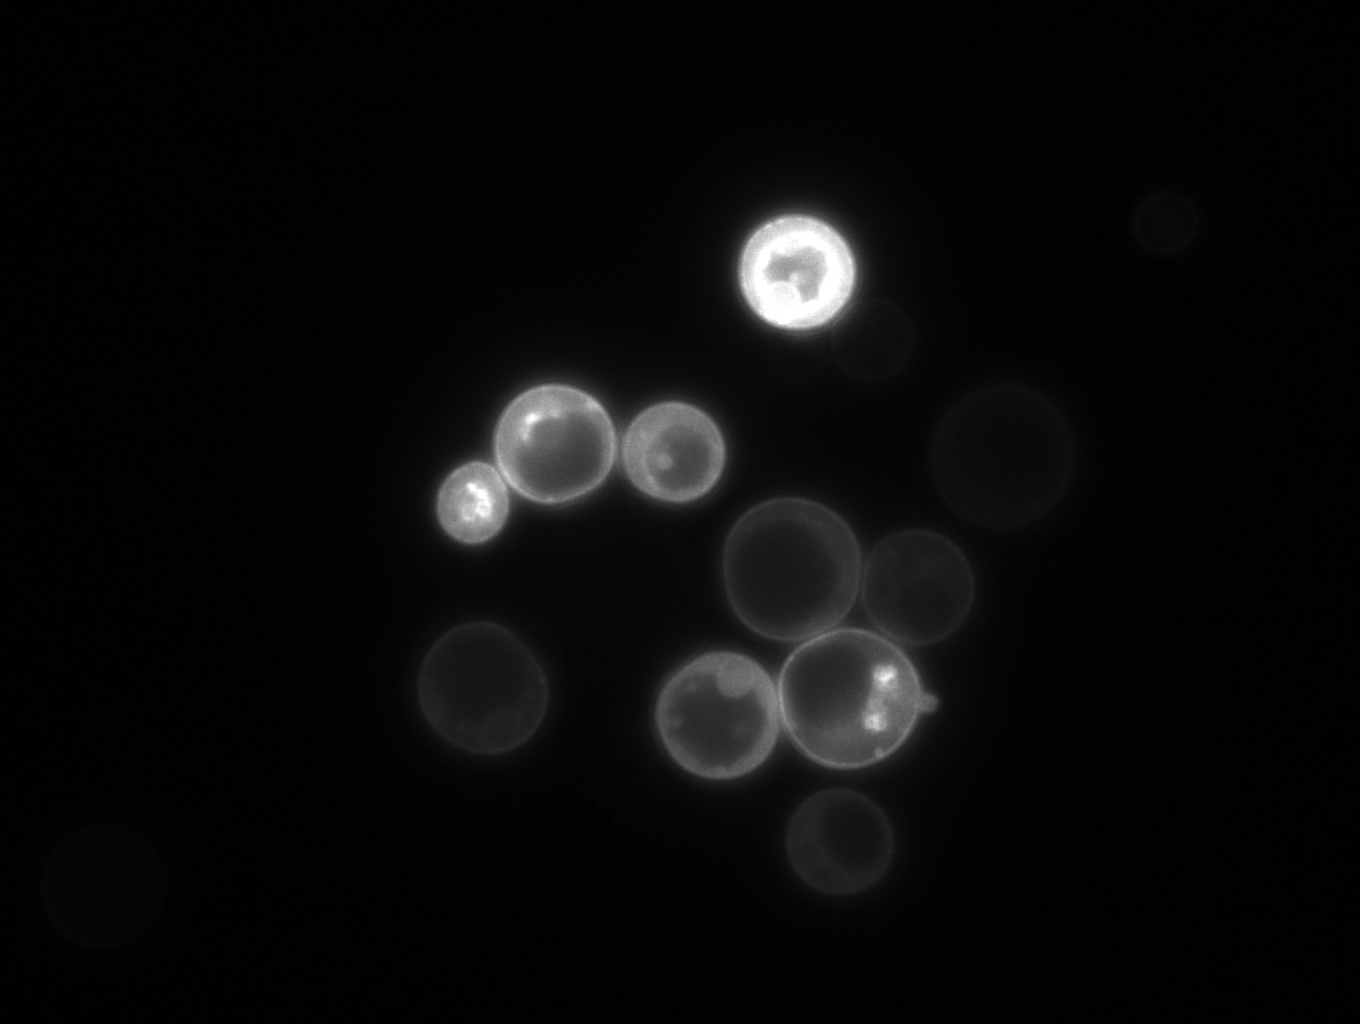
\includegraphics[width = \textwidth]{pics/1246_5hrs_GAL-4-1.png}
		\caption{Флуюресценция}\label{fig:}
	\end{subfigure}

	\caption{Экспрессия α-синуклеина-GFP штаммом W303/αSyn после индукции на галактозе в течении 5 часов.}
	\label{fig:fluo}	
\end{figure*}


\begin{figure*}[h]
	\centering

	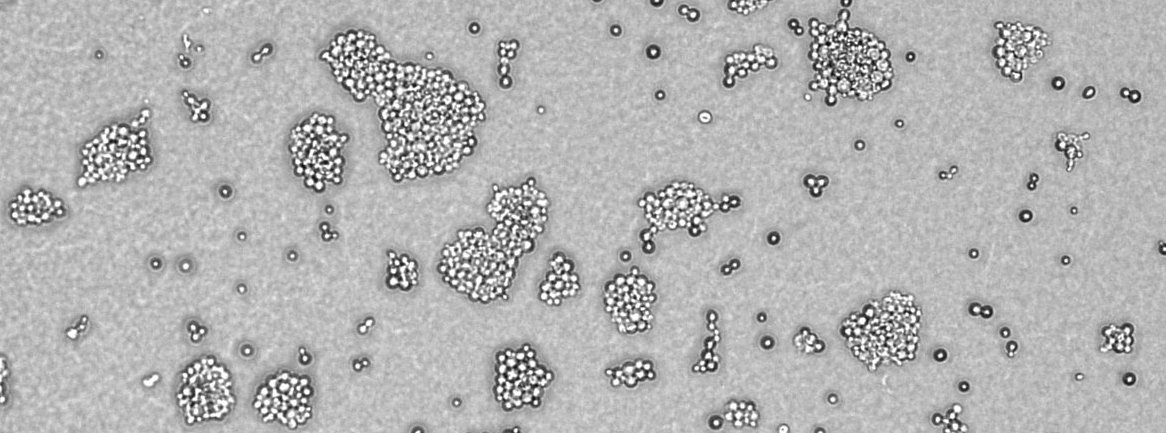
\includegraphics[width = 0.7\textwidth]{pics/16_4_1246_5_nghts_-uraGAL.jpg}
	\caption{Штамм W303/αSyn после культивирования на галактозе в течение 5 суток.}
	\label{fig:division}	
\end{figure*}

%\begin{figure*}[h]
%	\centering
%	\begin{subfigure}[t]{0.49\textwidth}
%		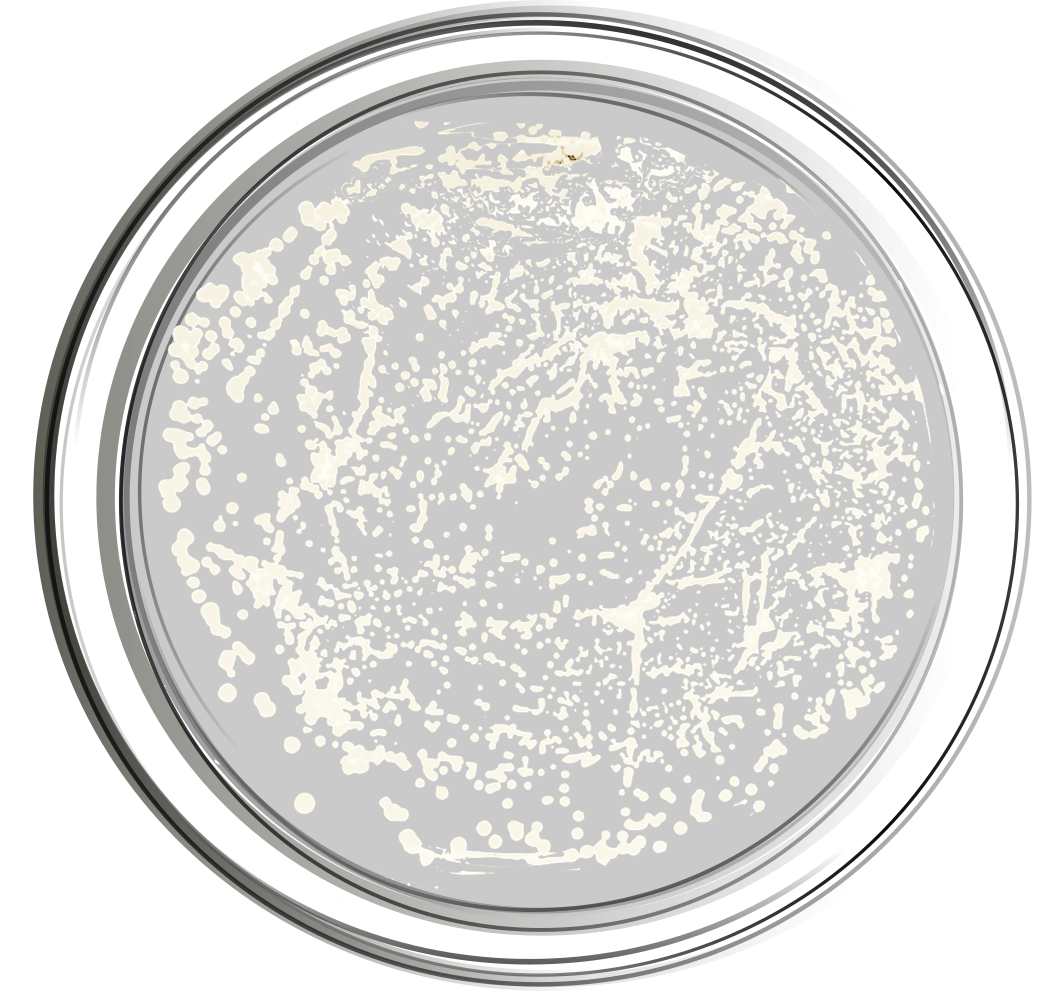
\includegraphics[width = \textwidth]{pics/1158_4n_glu_bw.png}
%		\caption{YNB-uraD}\label{fig:glu}
%
%	\end{subfigure}
%	\begin{subfigure}[t]{0.49\linewidth}
%		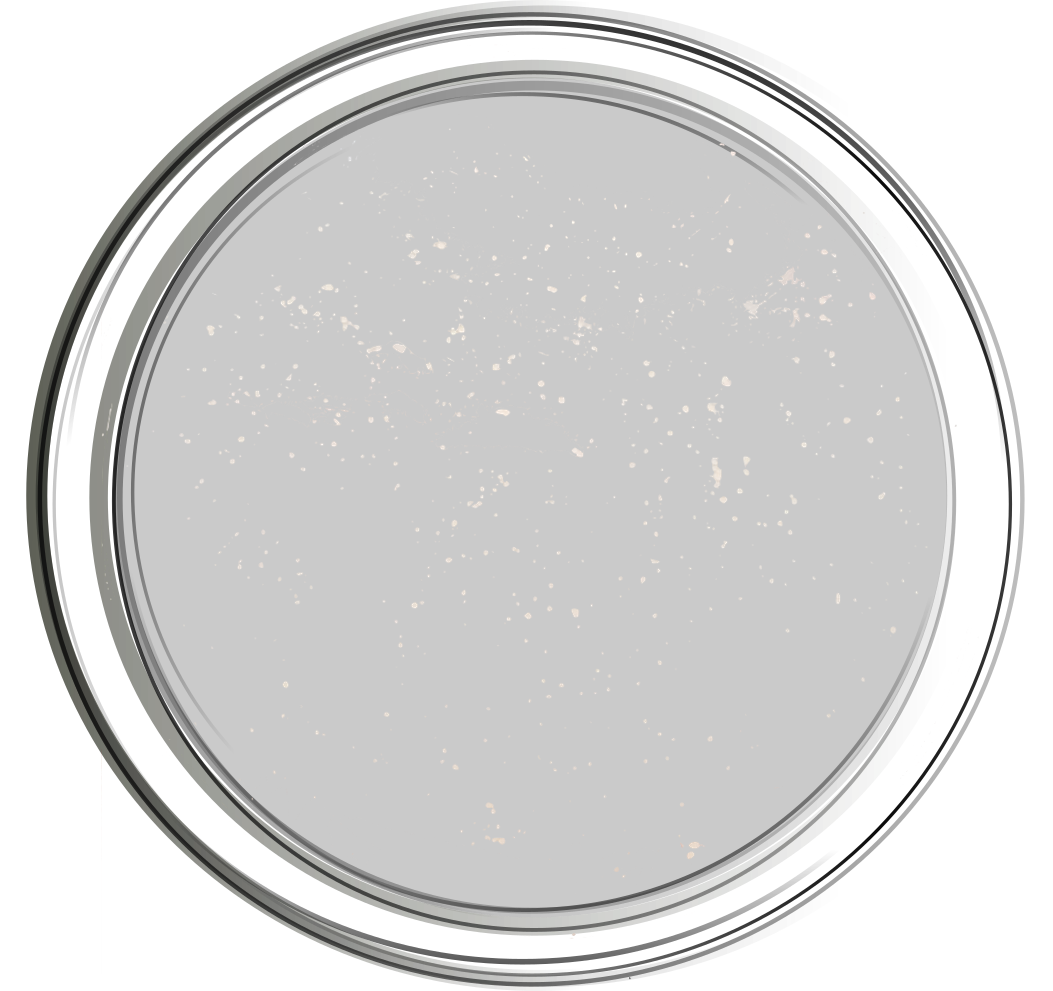
\includegraphics[width = \textwidth]{pics/1158_4n_gal_bw.png}
%		\caption{YNB-uraGAL}\label{fig:gal}
%	\end{subfigure}
%
%	\caption{
%	Рост штамма W303/αSyn: культивирование в течение 4 суток на средах: (a) с глюкозой и \ref{fig:gal} индуцирующей с галактозой. На глюкозе штамм формирует крупные колонии,на галактозе -- мелкие и в меньшем количестве. 
%	\gray{Картинки были созданы из фотографий чашек петри с помощью графических редакторов с сохранением формы и размера колоний для качественной иллюстрации}.
%		}
%	\label{fig:compare}	
%\end{figure*}



Оверэкспрессионная библиотека была трансформирована в штамм  W303/αSyn. Но не было получено ни одного клона. Трансформацию повторили, также с другими клонами W303/αSyn и штаммом, содержащим аналогичную плазмиду pYES-DA-6. При этом аналогичная процедура трансформации успешно проходила с дрожжами дикого типа W303 и штаммом W303:URA3.

Чем могло быть вызвано такое поведение штаммов W303/αSyn? Во-первых, какими-то процедурными неточностямии и ошибками, которые мы не смогли выявить. Во-вторых, мы предположили, что клетки не могут по каким-то причинам удержать обе плазмиды, которые мы хотели поместить в них, так они высококопийные. 

%Тогда мы решили интегрировать плазмиду p426GALaSynGFP и аналогичную по маркёру URA3 плазмиду pYES-DA-6 в геном дрожжей (см. \ref {subsec:integration}). 
%Было проанализировано 20 клонов для плазмиды p426GAlaSynGFP, 10 для плазмиды pYES-DA-6 с помощью ПЦР. Дополнительно, некоторые клоны были трансформировали оверэкспрессионной библиотекой. В результате клонов с встроившейся плазмидой и/или транформирующихся библиотекой найдено не было.
%Для преодоления данного препятствия было предложено несколько путей решения. Один из них заключался в использовании диплоидного штамма, клетки которого больше, содержат больше ДНК, в которых количественно больше машинерии для содержания ДНК-плазмид. Второй способ заключался с переносе интересующей конструкции в центромерную плазмиду pRS314. Эта плазмида в клетке реплицируется наряду с хромосомами и обычно очень низкокопийна.

Для решения этой проблемы было опробовано несколько подходов: (1) интеграция плазмид в геном, (2) проверка совмести мости плазмида с библиотекой в диплоидном штамме, (3) проверка совместимости плазмидного скелета pRS314 с оверэкспрессионной библиотекой.


%Диплоидный штамм был трансформирован плазмидой p426GAlaSynGFP, отобраны клоны, которые далее были транформированы оверэкспрессионной библиотекой, эффективность 60\,клонов/мкл.

%Плазмида pRS314, пока без интересующей конструкции, также были трансформирована в дрожии дикого типа W303, полученные клоны далее трансформированы оверэкспрессионной библиотекой, эффективность 30\,клонов/мкл.

Был заново проведен поиск клона W303/αSyn с более высоким уровнем токсичности α-синуклеина, выбран новый клон W303/αSyn, который, как оказалось, трансформировался оверэкспрессионной библиотекой.

Делеционная библиотека эффективно трансформировалась в штаммы.

Таким образом, мы получили штаммы W303/αSyn, cdc53-1/αSyn, которые экспрессируют α-синуклеин на галактозе, α-синуклеин для них токсичен и образует включения в клетках, которые трансформируются геномными библиотеками.




\subsection{Подбор стратегии скрининга для поиска генетических элементов, вовлеченных в токсичность α-синуклеина в дрожжах}

Мы планировали проводить скрининги на выживание на галактозе. После трансформации геномных библиотек в штаммы планировалось подобрать условия  процедуры так, чтобы после индукции экспрессии α-синуклеина, отбиралось около 0.1-0.5\% трансформантов. Более жесткие условия могли бы нивелировать разницу между разными моделями. С другой стороны, необходимо было понизить уровень ложно-положительных результатов -- отбора клонов, которые не получили никакого генетического преимущества и выросли случайно. Было предложено два варианта проведения скрининга -- с перепечатыванием и с непосредственнным высеванием на индуцирующую среду (см.~\ref{subsec:screening_strats})


Вариант процедуры скрининга с перепечатыванием был протестирован на штамме W303/αSyn с использованием делеционной библиотеки (см.~\ref{subsec:printing}).

Оказалось, что предложенный способ имеет недостатки: (1) размер колоний при перепечатывании очень важен, слишком мелкие колонии сложно все перенести на новую чашку, переросшие же колонии создают неравномерность -- разное количество клеток может быть перенесено, что может очень сильно повлиять на дальнейший рост, что противоречит выбранному критерию отбора; (2) после переноса доля выросших клонов оказалась слишком высокой -- около 10\% -- что говорит о неэффективности процедуры.

Был выбран второй вариант скрининга с непосредственным высеванием на индуцирующую среду (см.~\ref{subsec:immidiately}).

В рамках тестового скрининга мы провели серию транcформаций со штаммами W303/αSyn и cdc53-1/αSyn (при 25°C и 37°C). 
 В таблице~\ref{table:clones_stat} приведены: доля клонов, которые отбирались на галактозе, достигнутое покрытие генома при первичном отборе, предположительная клонов для проверки для полного покрытия генома.


\begin{table}[h]
	\caption{Характеристика первичного отбора, дотигнутого в скринингах.}
	\label{table:clones_stat}
	\begin{tabular}{
		p{0.2\width - \tabcolsep} 
		p{0.2\width - 2\tabcolsep} 
		R{0.2\width - 2\tabcolsep} 
		R{0.2\width - 2\tabcolsep}
		R{0.2\width - \tabcolsep}
		}
	\graytable
	\toprule
	 Штамм & Библиотека & Доля отбираемых клонов & Покрыто генома при первичном отборе & Клонов для проверки всего \\
	\midrule
	W303/αSyn & оверэкс. & 0,4\% & 75\%  & 40 \\
	W303/αSyn & делец. & 0,15\% & 7\% & 45 \\
	cdc53-1/αSyn & оверэкс. & 5\% & 10\% & 500\\
	cdc53-1/αSyn & оверэкс. (тепловой~шок) & 0,7\% & 45\% & 70\\
	\bottomrule
	\end{tabular}
\end{table}


Стоит заметить, что крупные колонии на галактозных чашках после трансформации W303/αSyn появлялись медленно, становились видимыми после 2 суток культивирования, отсаживались после 3-4.
В экспериментах с штаммом cdc53-1/αSyn это время было больше -- около 5-7  дней, так как штамм растет сам по себе очень медленно. После теплового больше колонии появились через 10 суток.
%Полученное время достаточно велико -- за него может произойти множество перестроек в клетке, которые мы не сможем оценить. Поэтому доверять большим колониям после 10 суток культивирования может быть неразумно.

%Выбранный критерий отбора оказался достаточно жестким в экспериментах со штаммом W303/αSyn, но для штамма cdc53-1/αSyn критерий оказался слишком мягким, так как доля отбираемых клонов составляет >0.5\%. 
%Поэтому условия скрининга для штамма cdc53-1/αSyn требуют ужесточения.

Итак, мы остановились на варианте проведения скрининга с непосредственным высеванием на индуцирующую среду. 

\subsection{Проверка клонов, прошедших отбор при скрининге}

Для дальнейшего анализа отобранных трансформантов нам было необходимо убедиться, что эффект повышения выживаемости значителен, воспроизводим и обусловлен делецией или оверэкспрессией какого-либо гена. 

%Воспроизводимость для оверэкспрессионной библиотеки можно было бы проверить выделением плазмиды, ее амплификацией, повторной трансформацией в дрожжи, проверкой.



Клоны, отобранные в результате трансформации штамма W303/αSyn оверэкспрессионной библиотекой были проверены на выживаемость и наличие GFP в клетке (см.~\ref{subsec:second_check}).

% Мы оценивали их скорость росте на галактозе по сравнению со штаммом W303/αSyn/LEU2 (негативный контроль) и W303::URA3/LEU2 (позитивный контроль), а также светимость GFP после индукции экспрессии. Было проверено 30 клонов. Оказалось, что не потерявшие целевую плазмиду клоны сильно уступают в скорости роста штамму W303::URA3/LEU2, и растут в некоторых случаях незначительно лучше W303/αSyn/LEU2. Один клон показал восстановление выживаемости, но он потерял токсичную плазмиду p426GALaSynGFP.


На данный момент нам не удалось обнаружить клонов, которые бы показали значительное и воспроизводимое повышение выживаемости. Было проверено 30 клонов для штамма W303/αSyn и оверэкспрессионной библиотеки, что покрывает около 75\% генома штамма.

Получается, что условия скрининга для штамма W303 оказались слишком жесткими, так при покрытии генома 75\% генетических элементов, повышающих выживаемость при экспрессии синуклеина найдено не было. 


\section{Выводы}


\begin{itemize}[label={--}]
	
\item был подготовлен ДНК-материал для трансформаций дрожжей \emph{Saccharomyces cerevisiae} -- оверэкспрессионная и делеционная дрожжевые геномные библиотеки;
\item созданы штаммы дрожжей \emph{Saccharomyces cerevisiae} W303 и cdc53-1 с индуцибельной экспрессией гибридного белка α-синуклеина-GFP;
\item показано, что α-синуклеин токсичен для штаммов W303 и cdc53-1;
%\item отработаны различные методики трансформации дрожжей;
\item начат скрининг, покрыто 75\% генома для штамма W303/αSyn и оверэкспрессионной библиотеки, клонов найдено не было;
\item показано, что условия скрининга нуждаются, с одной стороны, в смягчении, а с другой стороны -- в повышении эффективности поиска.
\end{itemize}






 




